\chapter{Previous Designs and Implementations}\label{sec:previous-designs}

Prior to my work on ShareTrace, I had no experience developing an algorithm that (at least hypothetically) required scalability. Ultimately, I implemented five designs of risk propagation, each providing insight that allowed for iterative improvement in performance. The following provides motivation and context for each design, along with rationale for pursuing an alternative approach.

\section{Thinking Like a Vertex}\label{sec:giraph}

%% TODO Add repo citation after code cleanup
%% TODO Cite TLOV
The first iteration of risk propagation utilized Apache Giraph \cite{Giraph2020}, an open-source version of the iterative graph-processing library, Pregel \cite{Malewicz2010}, which is based on the bulk synchronous parallel model for distributed computing \cite{Valiant1990}. Giraph follows the think-like-a-vertex paradiagm for graph-processing algorithms in which the algorithm is specified from the perspective of a vertex. As a highly scalable framework for graph-based algorithms, Giraph was a natural choice for implementing risk propagation. Figure \ref{fig:v1-architecture} describes the full compute architecture.

\begin{figure}[htbp]
\centering
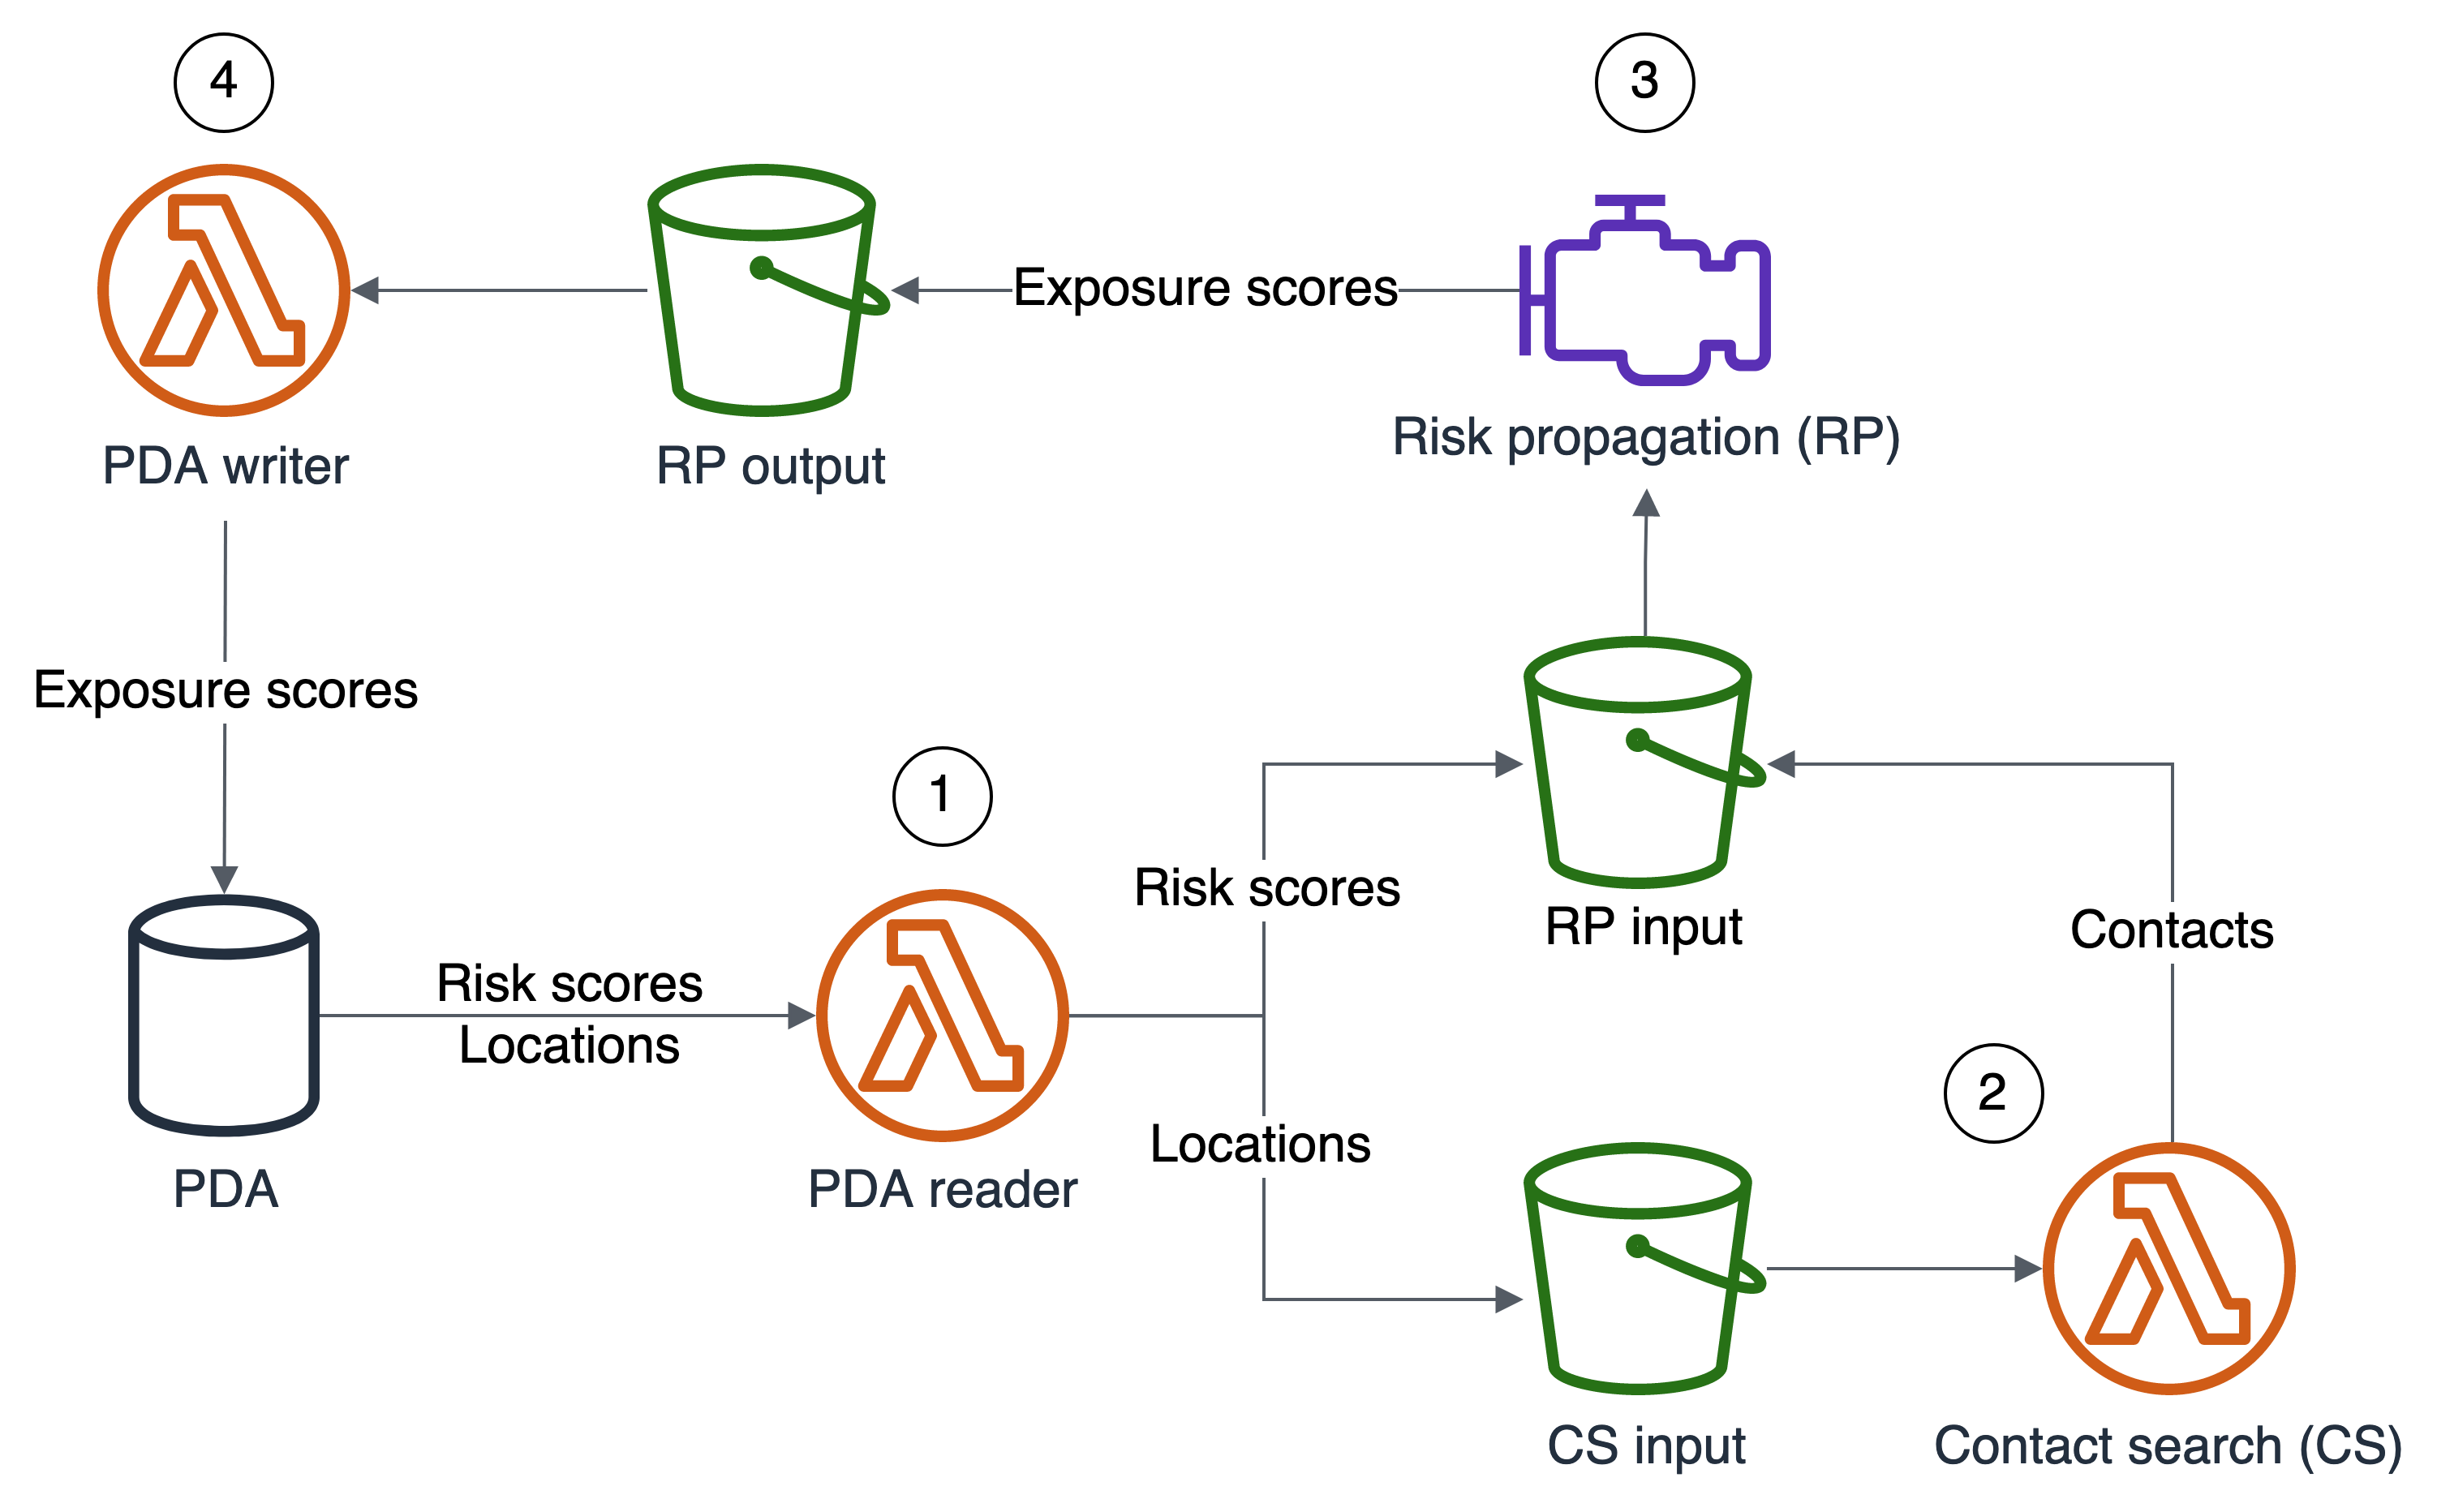
\includegraphics[width=\textwidth]{v1-architecture}
\caption[ShareTrace batch-processing architecture]{ShareShareTrace batch-processing architecture.
(1) An AWS Lambda function retrieves the risk scores (symptom scores and previously computed exposure scores) and location histories from all user PDAs. Risk scores are transformed into vertex inputs for risk propagation and stored in an Amazon Simple Service (S3) bucket. Location histories are stored in a separate S3 bucket for contact extraction. (2) An AWS Lambda function executes contact search on the location histories to find all contacts, maps them to edge inputs for risk propagation, and stores them in the same S3 bucket that holds the vertex inputs. (3) Amazon Elastic MapReduce (EMR) runs risk propagation as a batch job and outputs the computed exposure scores into an S3 bucket. (4) An AWS Lambda function writes the exposure scores to the PDA of their respective user.}
\label{fig:v1-architecture}
\end{figure}

%% TODO Cite AWS Batch, S3, EMR, Lambda, Step Function
%% TODO Cite fan-out pattern
The functionality implemented by all AWS Lambda functions was intended to follow a fan-out design in which one Lambda function would be invoked and then distribute the work amongst one or more other Lambda functions. For example, the PDA reader Lambda function would retrieve the list of all HATs and then partition that list among several other Lambda functions to retrieve user data in parallel.

The Giraph-based implementation is a literal interpretation of the original ShareTrace algorithm \cite{Ayday2021}. That is, it assumes a factor graph in which a factor vertex contains the contact times between two users and a variable vertex contains the maximum risk score it has received from a neighboring factor vertex. The algorithm haults when either a given number of iterations has elapsed or the total change in variable vertex values drops below a given threshold.

Several factors prompted the search for an alternative design to Giraph:
\begin{enumerate}
\item \emph{Design complexity}. For a relatively straightforward data flow, the architecture in Figure \ref{fig:v1-architecture} corresponds to over 4,000 lines of source code. In retrospect, a more suitable approach than manually configured Lambda  functions would have been a managed batch-processing or workflow orchestration service, such as AWS Batch or AWS Step Function. Additionally, the low-level design of the Giraph implementation was unnecessarily complex. One-mode projection that is used in Sections \ref{sec:projected-subgraphs} and \ref{sec:vertex-actors} would have avoided the complexity of multiple vertex types. Regardless, the implementation was overengineered.
\item \emph{Dependency management incompatability}. A major cause for redesigning the implementation was the dependency version conflicts between Giraph and the libraries used for the ShareTrace implementation. In spite of the several attempts (e.g., using different library versions, using different versions of Giraph, and forcing specific transitive dependency versions) to resolve these conflicts, a lack of personal development experience and stalled progress prompted me pursue alternatives to Giraph.
\item \emph{Persistent data storage external to the PDA}. One of the core tenets of Dataswift is that the user fully controls the access to their data. However, as shown in Figure \ref{fig:v1-architecture}, user data is stored in S3 buckets. While it is possible to encrypt S3 objects at rest and automatically delete objects after a certain duration, data persistence to any extent is neither ideal nor desired for a privacy-preserving contact tracing solution.
\end{enumerate}

%% TODO Cite Plasma object store
%% TODO Cite GitHub repo after code clean up
\section{Subgraph Actors}\label{sec:subgraph-actors}

Attempting to mimic the design in Section \ref{sec:giraph}, I implemented risk propagation using the Python library, Ray  \cite{ray2021} that ``provides a simple, universal API for building distributed applications.'' While it claims to support actor-based programming, Ray provides relatively basic support compared to Akka, which is used in the current implementation (see Section \ref{sec:vertex-actors}). Essentially, Ray offers an extension of multiprocessing in which each actor is bound to a process. For risk propagation, I partitioned the factor graph among multiple actors such that each actor maintained a subset of variable vertices \emph{or} factor vertices. The graph topology was stored in shared memory so that it all actors could efficiently access it. The lifetime of this design was brief for the following reasons:

\begin{enumerate}
\item \emph{Poor performance}. Interprocess communication is relatively more expensive than intraprocess communication. As a result, by partitioning the vertices such that actors only contained one type of vertex in the bipartite graph, all messages passed during risk propagation were sent to different processes. Unsurprisingly, this manifested in slow runtimes.
\item \emph{Design complexity}. Not using a framework, like Giraph, meant that this implementation required more low-level code to implement actor functionality and message-passing. Regardless of the performance, the overall design of this implementation was poorly organized and overthought.
\end{enumerate}

\section{Monitor-Worker-Driver (MWD) Framework}\label{sec:monitor-worker}

% TODO Cite https://docs.ray.io/en/latest/ray-core/actors/patterns/tree-of-actors.html
% TODO Cite https://docs.ray.io/en/latest/ray-core/tasks/patterns/fine-grained-tasks.html
Based on the poor runtime performance and complexity of the approach taken in Section \ref{sec:subgraph-actors}, I speculated that centralizing the mutable aspects of risk propagation (i.e., the current value of each variable vertex) would decrease runtime and reduce the implementation complexity. With this is mind, I designed the monitor-worker-driver (MWD) framework, which draws inspiration from the tree of actors design pattern [CITE].  Figure \ref{fig:v3-architecture} describes the framework. Listing \ref{listing:v3-code} provides a partial implementation of the monitor and driver.

\begin{figure}[htbp]
\centering
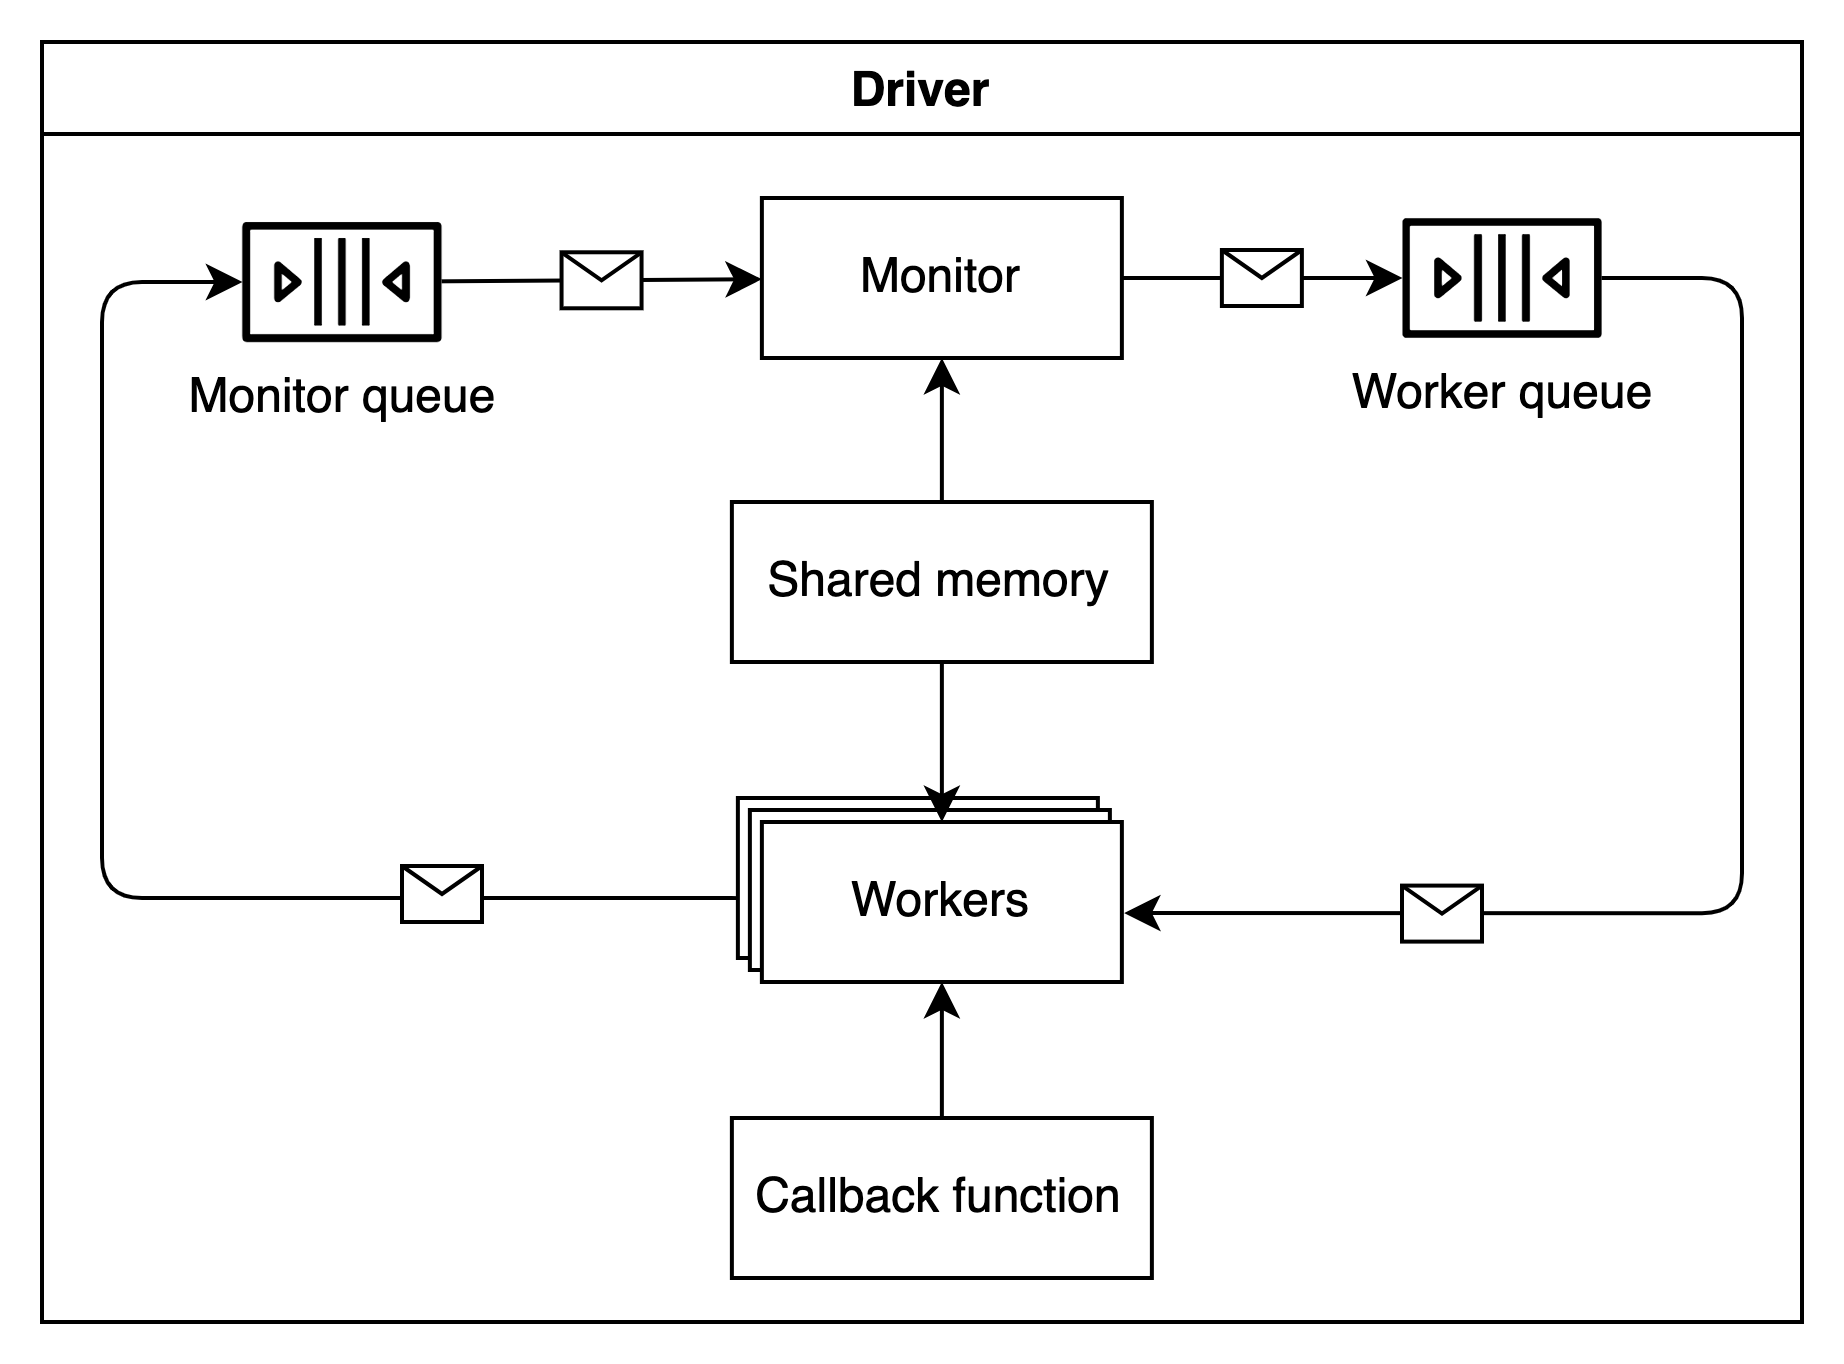
\includegraphics[width=\textwidth]{v3-architecture}
\caption[Monitor-worker-driver framework]{Monitor-worker-driver framework.
The \emph{monitor} is a stateful actor that is responsible for any mutable state of the program. A \emph{worker} (e.g., threads, processes, etc.) is a stateless entity that consumes monitor-produced messages from the \emph{worker queue}. Following the strategy design pattern \cite{Gamma1994}, worker behavior is defined by a \emph{callback function} which may use the attributes of a message to decide on how to process it. Any side effects of processing a message from the worker queue is encapsulated in a message and added to the \emph{monitor queue}. The monitor then consumes messages from the monitor queue, updates the state of the program, and produces messages in response for the workers to consume. The use of queues follows the mediator design pattern \cite{Gamma1994} in that the monitor and workers communicate indirectly. Any immutable state of the program can be efficiently accessed by both the monitor and the workers in \emph{shared memory}. The \emph{driver} is responsible for initiating the monitor and workers, waiting for the monitor to terminate message-passing, and returning the program output.}
\label{fig:v3-architecture}
\end{figure}

\begin{figure}[htbp]
\centering
\begin{lstlisting}[
caption={[Monitor-worker-driver framework code]Monitor-worker framework code. The \texttt{BaseMonitor} is responsible for observing the message-passing between workers and maintaining any state of the program. The \texttt{BaseDriver} defines the rest of the message-passing program by first completing any required setup, and then returning the result from the monitor. It is composed of a worker queue instance, a monitor queue instance, a worker callback function, and the number of workers to instantiate. The type variables \texttt{Q} and \texttt{M} are used to indicate the types of the queue and message, respectively. The \texttt{BaseMonitor.call(Q, Q)} method follows the template design pattern in that it specifies the composition of multiple abstract methods and leaves their implementation to subclasses \cite{Gamma1994}.},
label=listing:v3-code]
from abc from ABC
from typing import Any, TypeVar

Q, M = TypeVar("Q"), TypeVar("M")

class BaseMonitor(ABC):
    __slots__ = ()

    def call(self, mqueue: Q, wqueue: Q) -> Any:
        while not self.should_terminate():
            # Get a message from the monitor queue.
            msg = self.get(mqueue)
            # Only process the message if necessary.
            if self.should_process(msg):
                # Optionally modify the message.
                msg = self.transform(msg)
                # Update the state of the monitor.
                self.update(msg)
                # Put the message in the worker queue.
                self.put(wqueue, msg)

class BaseDriver(ABC):
    __slots__ = "monitor", "mqueue", "wqueue", "callback", "n_workers"

    def call(self, inputs: Any) -> Any:
        # Perform any necessary setup before starting.
        self.setup(inputs)
        return self.monitor.call(self.mqueue, self.wqueue)
	\end{lstlisting}
\end{figure}

For risk propagation, a \texttt{RiskMonitor} monitor was implemented. It terminates when any of the following conditions are satisifed. The default behavior is to terminate once the monitor queue is empty.

\begin{itemize}
	\item The monitor has received \texttt{max\_msgs} messages.
	\item A duration of \texttt{max\_duration} has elapsed.
	\item No variable vertex has updated after \texttt{n\_msgs\_early\_stop} messages.
	\item No messages have been received \texttt{n\_retries} times after \texttt{timeout} time.
\end{itemize}

Only messages that are likely to induce an update to the state of the monitor are processed. The \texttt{send\_threshold} parameter allows us to vary the strictness of this likelihood. For a message sent by a variable node, the monitor only allows it if the value, scaled by \texttt{send\_threshold}, is greater than the current value of the variable vertex. This does not guarantee that it will invoke an update after the receiving factor vertex processes it, but it does prevent messages that would obviously not cause a variable vertex to update its value. Similarly, for a factor message, the monitor only allows it if the value, scaled by \texttt{send\_threshold}, is greater than the current value of the receiving variable vertex. Unlike variable messages, this guarantees against sending ineffective messages. Even if no other terminating condition is specified, the nature of \texttt{filter(M)} will gradually cause message passing to terminate. No transformation is applied to messages. The \texttt{update(M)} method contains the logic corresponding to the terminating conditions specified earlier. The monitor also updates the value of a variable vertex if the message value is greater than its current value.

The \texttt{RiskPropagation} driver exectutes risk propagation. Its \texttt{setup(Any)} method (1) creates the factor graph and stores it in shared memory, (2) sets the initial state of the monitor to be the maximum risk score of each variable vertex, and (3) adds all risk scores to the monitor queue. The \texttt{call(Any)} method (1) calls \texttt{setup(Any)}, (2) initializes \texttt{n\_workers} workers and the monitor, and (3) returns the state of the monitor, which is the exposure score of variable vertex.

Compared to the approach in Section \ref{sec:subgraph-actors}, this implementation provides a cleaner design and less communication overhead. However, what prompted me to consider (yet another) an alternative implementation was its scalability. As evidenced by Listing \ref{listing:v3-code}, the MWD framework is just a way of organizing an algorithm around the monitor while loop. Because the monitor processes messages serially, it is a bottleneck for algorithms in which the workers perform fine-grained tasks. Indeed, the Ray documentation notes that the parallelization of small tasks is an antipattern because the interprocess communication cost exceeds the benefit of multiprocessing [CITE]. Unfortunately, the functionality of a variable vertex and factor vertex is too fine-grained, so the scalability of the MWD framework is no better than a serial implementation.

% TODO Mention adjacency-list representation of the graph
\section{Subnetwork Actors with Projection}\label{sec:projected-subgraphs}
%Improvements:
%1. Best functioning implementation thus far
%
%Drawbacks:
%1. Heavily dependent on the graph partitioning – load balancing and communication overhead


% TODO Move this into main chapter
\section{Thinking Like a Vertex with Actors}\label{sec:vertex-actors}

Improvements:
1. Distributed; a drawback of all but the first approach
2. Decentralized; a drawback of all previous approaches
3. Robust; allows for delays in the changes of the contact graph with caching
4. Scalable and performant

Drawbacks:
1. Concurrent execution is difficult to reason about

\section{Location-Based Contact Tracing}\label{sec:location-based}
	\begin{itemize}
	\item Motivation: Google/Apple API prevents exporting Bluetooth EphIDs
	\item Other location-based contact tracing approaches
	\end{itemize}
\subsection{System Model}
The system model is very similar to previous work \cite{Ayday2020, Ayday2021} and designs. The only difference is that user geolocation data is collected instead of Bluetooth ephemeral identifiers. \Cref{fig:location-based} shows the modified dataflow\footnote{See \cref{foot:dataflow} (p. \labelcpageref{foot:dataflow}) for the definition of a dataflow diagram.}.
	\begin{figure}[ht!]
		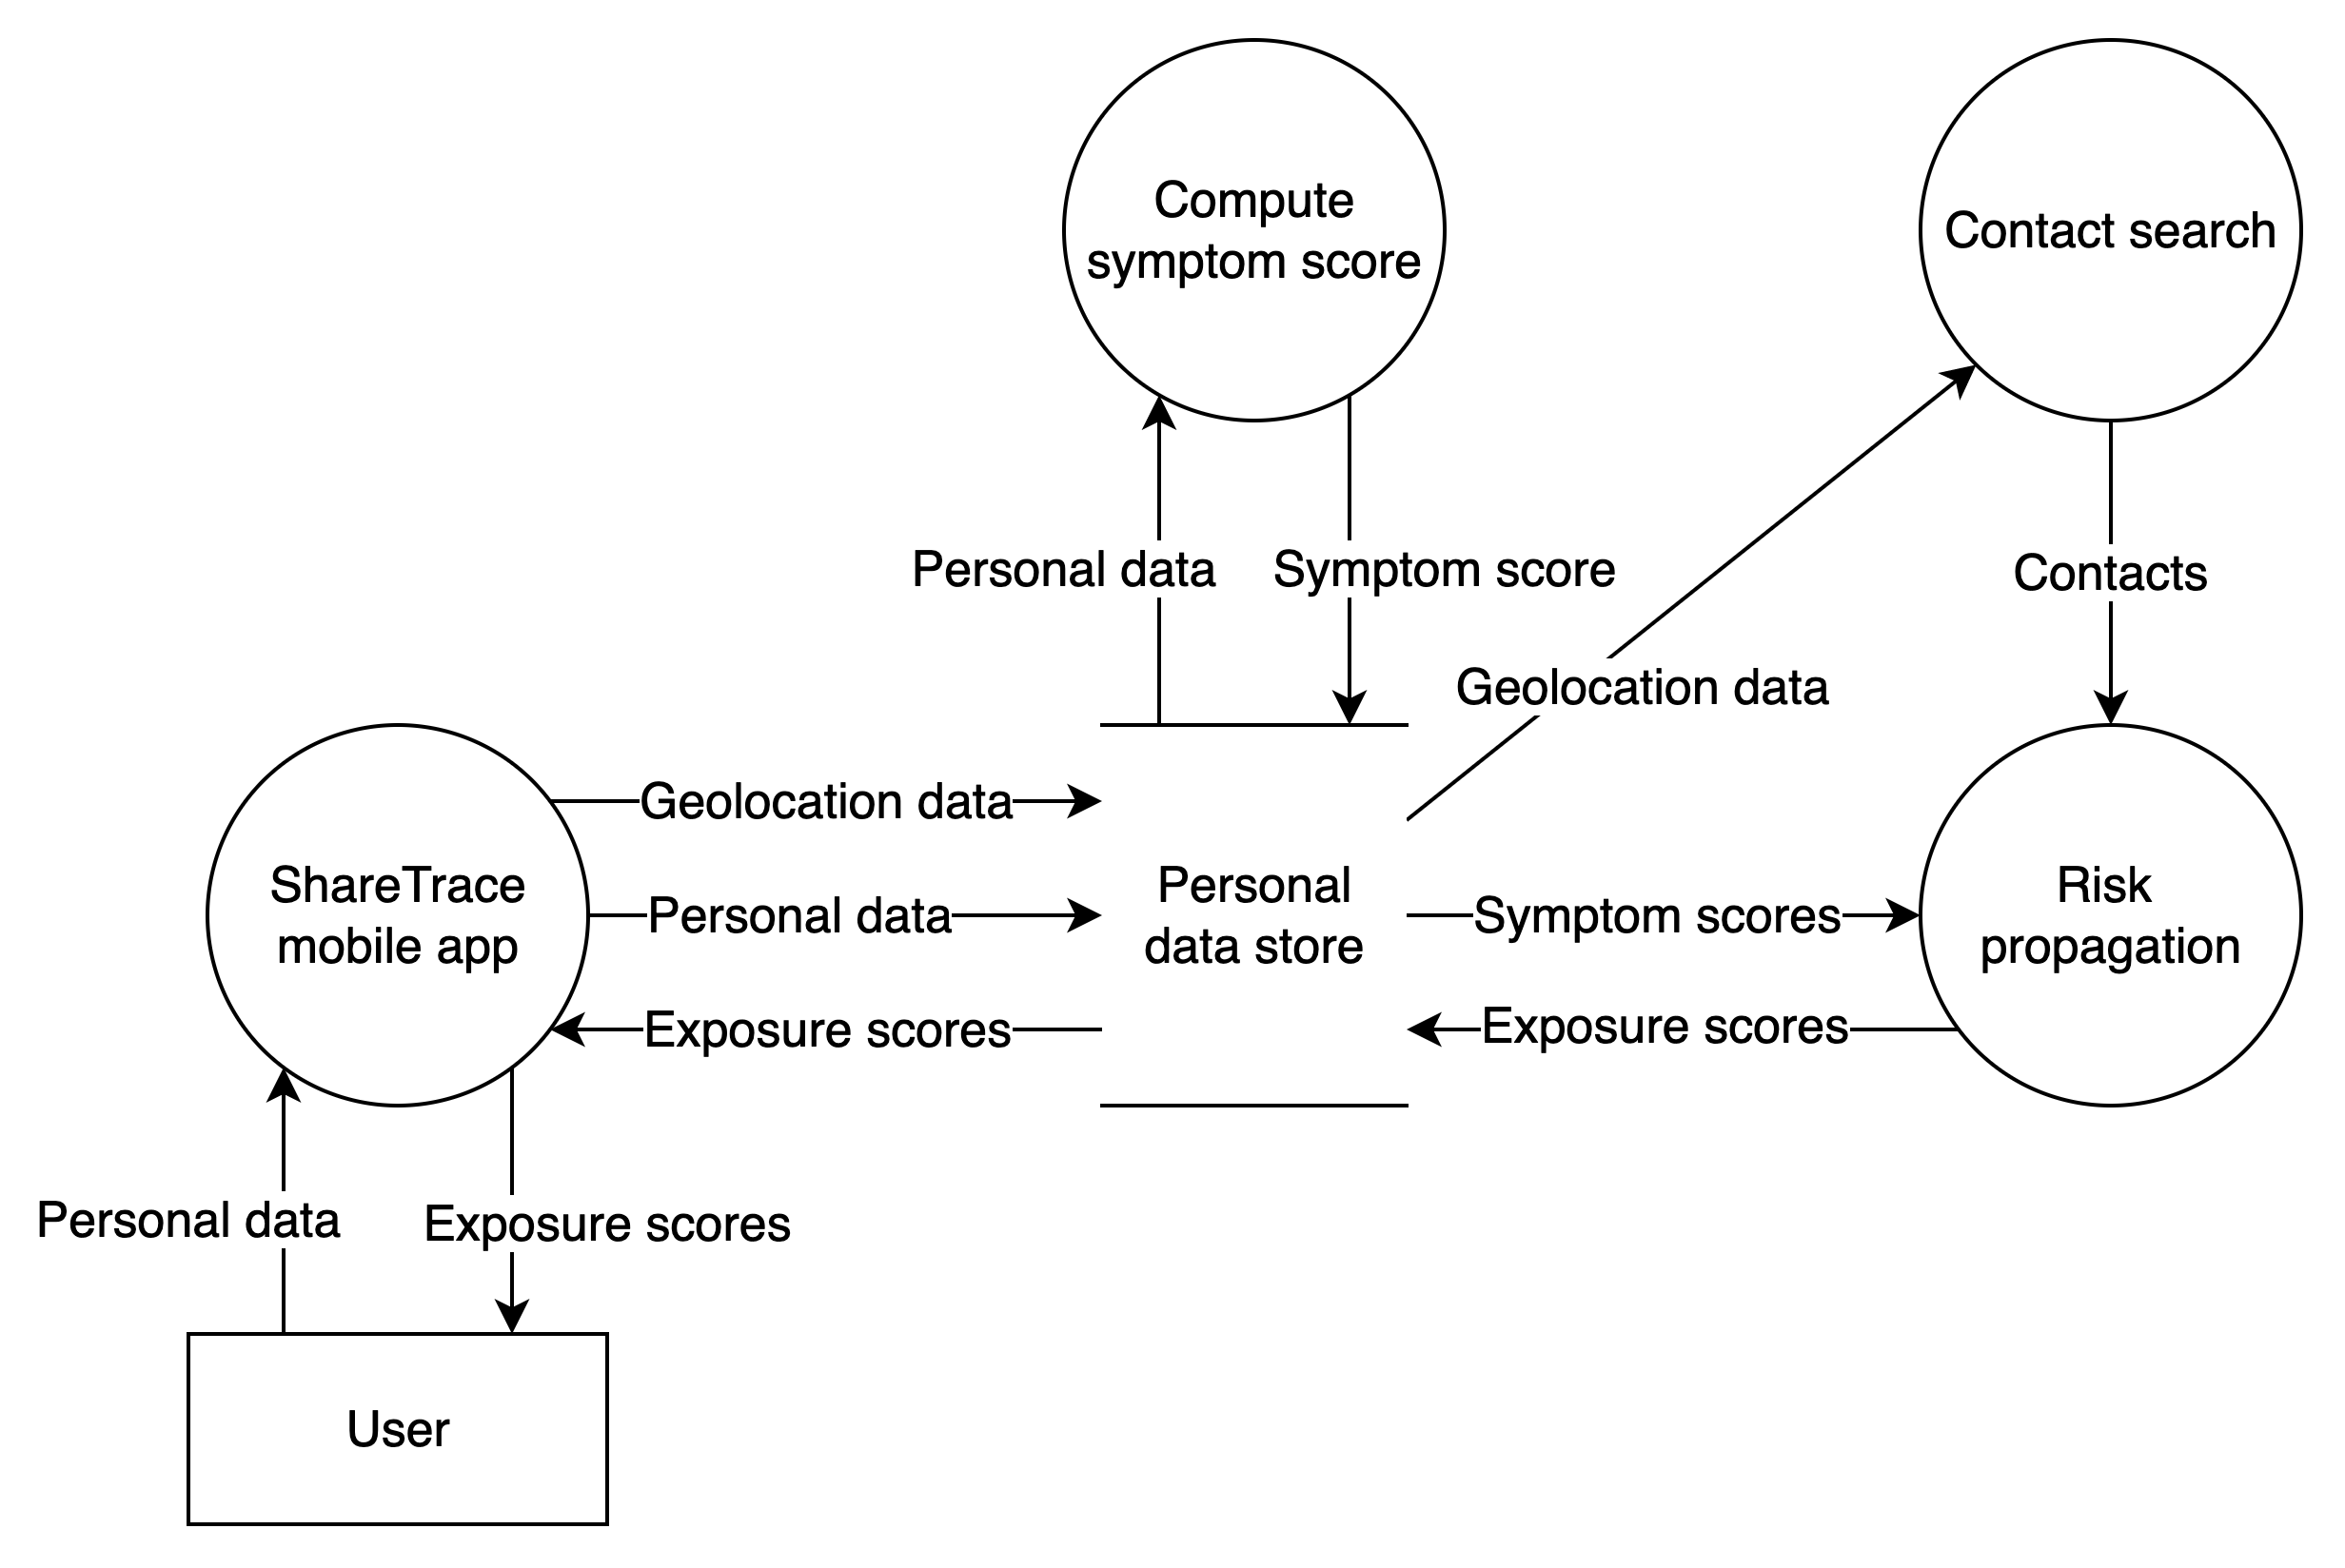
\includegraphics[width=\textwidth]{location-dataflow}
		\caption[Geolocation-based ShareTrace dataflow]{Location\hyp{}based ShareTrace dataflow. This requires that risk propagation is executed in a centralized setting since all user geolocation data is needed to construct the contact network.}
		\label{fig:location-based}
	\end{figure}
\emph{Geohashing} is a public\hyp{}domain encoding system that maps \emph{geographic coordinates} (i.e., latitude\hyp{}longitude ordered pairs \cite[p. 5]{Sickle2004}) to alphanumeric strings called \emph{geohashes}, where the length of a geohash is correlated with its geospatial precision \cite{Morton1966}. To offer some basic privacy, a user's precise geolocation history is obfuscated on\hyp{}device by encoding geographic coordinates as geohashes with 8\hyp{}character precision which corresponds to a region of $730\mathrm{m}^2$.

\subsection{Contact Search}
\newcommand{\histories}{\mathcal{H}}
\newcommand{\locations}{\mathbb{L}}
\newcommand{\locset}{\mathcal{L}}
\newcommand{\latitude}{\phi}
\newcommand{\longitude}{\lambda}
\newcommand{\users}{\mathcal{U}}
\newcommand{\sindex}{\mathcal{I}}
\newcommand{\query}{\mathcal{N}}
\newcommand{\qelement}{q}
\newcommand{\hone}{G}
\newcommand{\htwo}{H}
\newcommand{\neighbors}{N}
A \emph{contact} follows the definition of \eqref{eq:contact-seq}, where the contact time $\tsym$ indicates the most recent time at which two users were proximal for a contiguous duration of at least $\delta \in \preals$. Each user has a \emph{geolocation history}
	\begin{equation*}
		\htwo = \left[(\tsym_i, \ell_i) \mid ~\forall i \in \ints_{[1, \attr{\htwo}{length}]} (\tsym_i < \tsym_{i + 1}) \right],
	\end{equation*}
a temporally ordered sequence of timestamped geolocations. It is assumed that
	\begin{enumerate}
		\item geolocation histories are not recorded on a fixed schedule, and \label{assume:sched}
		\item a user remains at a geolocation until the next geolocation is recorded. \label{assume:static}
	\end{enumerate}
By assumption \ref{assume:sched}, any two geolocation histories can be ``out of alignment'' such that they are of different length with interleaving timestamps. Geolocation histories $\hone, \htwo$ can be \emph{aligned} by \emph{padding} such that
	\begin{equation*}
		n = \attr{\hone}{length} = \attr{\htwo}{length},
	\end{equation*}
and \emph{temporally interpolating} such that
	\begin{equation*}
		\forall i \in \ints_{[1, n]}(\timeAttr{\hone[i]} = \timeAttr{\htwo[i]}).
	\end{equation*}
By assumption \ref{assume:static}, it is most appropriate to use \emph{previous interpolation}: given timestamped geolocations $(\tsym_i, \ell_i), (\tsym_j, \ell_j)$ such that $\tsym_i < \tsym_j$, all intermediate geolocations are defined as $(\tsym_k, \ell_i)$ for all $\tsym_k \in [\tsym_i, \tsym_j)$. In practice, time is a discrete variable that is recorded with fixed precision (e.g., seconds). Let $T \in \pints$ be the \emph{time period} between two consecutive timestamps $\tsym_i, \tsym_{i + 1}$ such that $\tsym_{i + 1} = \tsym_i + T$. Then previous interpolation between timestamps $\tsym_i, \tsym_j$ such that $\tsym_j > \tsym_i$ results in $T \cdot (\tsym_j - \tsym_i - 1)$ intermediate geolocations.

Finding the most recent contact between two users from their aligned geolocation histories is similar to finding the last $k$\hyp{}length common substring between two strings, where each symbol represents a timestamped geolocation. The difference lies in how the start and end of the contact time interval is defined. By assumption \ref{assume:static}, the start (end) of a contact time interval is defined as the earlier (ref. later) timestamp of the two first (ref. last) timestamped geolocations in the sequence where the two histories differ. \Cref{fig:contact-search} provides a visual example.
	\begin{figure}[ht!]
	    \centering
	    \begin{tikzpicture}[scale=2]
	        \draw[latex-latex] (-3,0) -- (3,0);
	        \draw[latex-latex] (-3, 1) -- (3,1);
	        \draw (-2,0) -- (-2,1);
	        \draw (-1.5,0) -- (-1.5,1);
	        \draw (0.5,0) -- (0.5,1);
	        \draw (2,0) -- (2,1);
	        \draw (-1.75, 0.5) node {$A$};
	        \draw (1.25, 0.5) node {$B$};

	        \path [draw=black, fill=black] (-2,0) circle (1pt);
	        \path [draw=black, fill=black] (0,0) circle (1pt);
	        \path [draw=black, fill=black] (2,0) circle (1pt);
	        \path [draw=black, fill=black] (-2.5,1) circle (1pt);
	        \path [draw=black, fill=black] (-1.5,1) circle (1pt);
	        \path [draw=black, fill=black] (0.5,1) circle (1pt);
	        \path [draw=black, fill=black] (2.5,1) circle (1pt);

	        \node[below=2pt of {(-2,0)}] {$\ell_1$};
	        \node[below=2pt of {(0,0)}] {$\ell_3$};
	        \node[below=2pt of {(2,0)}] {$\ell_2$};
	        \node[above=2pt of {(-2.5,1)}] {$\ell_1$};
	        \node[above=2pt of {(-1.5,1)}] {$\ell_2$};
	        \node[above=2pt of {(0.5,1)}] {$\ell_3$};
	        \node[above=2pt of {(2.5,1)}] {$\ell_1$};
	    \end{tikzpicture}
	    \caption[Contact search with two geolocation histories]{Contact search with two geolocation histories. Each line denotes time, increasing from left to right. A point $\ell_i$ is a geolocation and occurs relative in time with respect to the placement of other points. Region $B$ defines the contact interval as it is of sufficient duration and occurs after $A$.}
	    \label{fig:contact-search}
	    \end{figure}

\subsubsection{Naive Contact Search}
A naive approach to finding all contacts amongst a set of geolocation histories $\histories$ is to compare all unordered pairs. For a given pair of aligned geolocation histories, the idea is to maintain a pointer to the previous and current index in each history, advancing the pair of pointers whose geolocation occurs later in time. Once a common geolocation is found, all pointers are advanced together until the geolocations differ. If the sequence is $\delta$\hyp{}contiguous, where a sequence of timestamped geolocations $S$ is \emph{$\delta$\hyp{}contiguous} if $\attr{S}{length} \geq \delta$ and
	\begin{equation*}
		\forall i \in \ints_{[1, \attr{S}{length}]}(\timeAttr{S[i + 1]} = \timeAttr{S[i]} + T),
	\end{equation*}
then it is recorded. The latest such sequence is used to define the contact between the two users. Because only the most recent time of contact is of interest, the procedure can be improved by iterating in reverse and then terminating once a sequence is found. Regardless, this approach takes $\Theta(n^2)$ time, where $n = \card{\histories}$, because all $\frac{n(n - 1)}{2}$ unique pairs must be considered.

The \Call{Naive\hyp{}Contact\hyp{}Search}{} operation implements the above procedure. The operation \Call{Most\hyp{}Recent\hyp{}Contact}{} considers geolocations\footnote{The symbol ``$\locations$'' denotes the space of all geolocations.} $\ell_i, \ell_j \in \locations$ \emph{$\epsilon$\hyp{}proximal} (i.e., approximately equal) if $d(\ell_i, \ell_j) \leq \epsilon$, according to some \emph{metric} $d: \locations \times \locations \rightarrow \nnreals$ \cite[p. 118]{Kelley1975} and distance $\epsilon \in \nnreals$. Because geolocations are encoded as geohashes, they must be decoded into geographic coordinates to perform this proximity calculation. Moreover, because geohashing discretizes the coordinate system into a grid of geographic regions, the number of possible geolocations is finite. Thus, the operation returns a $\delta$\hyp{}contiguous, $\epsilon$\hyp{}proximal contact $c$ if such a contact exists between the geolocation histories $\hone, \htwo \in \histories$. The \Call{Align\hyp{}Histories}{} operation pads each geolocation history such that the padded values (e.g., $\pm \infty$) do not result in false contact between users.
	\begin{algorithm}[ht!]
	\begin{algorithmic}[1]
		\Title{Naive-Contact-Search}{\histories}
		\State $\contacts \assign \emptyset$
		\ForEach{$(\hone, \htwo) \in \Call{Unique-Pairs}{\histories}$}
			\State $(\hone, \htwo) \assign \Call{Align-Histories}{\hone, \htwo}$
			\State $\var{c} \assign \Call{Most-Recent-Contact}{\hone, \htwo, \epsilon, \delta}$
			\If{$\var{c} \notequals \nil$}
				\State $\contacts \assign \contacts \cup \{c\}$
			\EndIf
		\EndFor
		\State \Return $\contacts$
	\end{algorithmic}
	\end{algorithm}

\subsubsection{Indexed Contact Search}
While the \textbf{for} loop in \Call{Naive\hyp{}Contact\hyp{}Search}{} is \emph{embarrassingly parallel} \cite[p. 14]{Herlihy2012}, the naive approach is neither scalable nor efficient. It can be improved by observing that it is necessary, but not sufficient, that a pair of $\epsilon$\hyp{}proximal geolocations exists between two geolocation histories for a contact to exist. Therefore, the geolocation histories $\histories$ can be indexed into a spatial data structure $\sindex$ \cite{Mokbel2003, Dinh2010, Mahmood2019} and then only consider the geolocation\hyp{}history pairs that share at least one $\epsilon$\hyp{}proximal geolocation pair. This approach is described by the \Call{Indexed\hyp{}Contact\hyp{}Search}{} operation.

Line \ref{step:query} executes a fixed\hyp{}radius near\hyp{}neighbors search (FR-NNS) \cite{Bentley1975, Brin1995} for each geolocation in the spatial index $\sindex$. Formally, given a set of geolocations $\locset \subseteq \locations$, a metric $d$, and a distance $\epsilon$, the \emph{fixed\hyp{}radius near\hyp{}neighbors} of a geolocation $\ell \in \locset$ is defined as the subset of $\epsilon$-proximal geolocations \cite{Brin1995},
	\begin{equation*}
		\query(\ell) = \{\ell' \in \locset \mid d(\ell, \ell') \leq \epsilon\}
	\end{equation*}

Note that the set of neighbors $\query(i)$ of user $i$ corresponds to the geolocations that are $\epsilon$\hyp{}proximal to \emph{any} of the geolocations in their geolocation history $\htwo_i$,
	\begin{equation*}
		\query(i) = \bigcup_{\ell \in \htwo_i} \query(\ell).
	\end{equation*}
On line \ref{step:to-users}, the operation \Call{Unique-Users}{} maps these near-neighbors back to the associated users, removing any duplicates that may arise from mapping multiple geolocations to the same user. Finally, line \ref{step:subset} maps the set of users $\users$ back to their geolocation histories and runs \Call{Naive-Contact-Search}{} on the resultant subset.
	\begin{algorithm}[ht!]
	\begin{algorithmic}[1]
		\Title{Indexed-Contact-Search}{\histories}
		\State $\sindex \assign \Call{Spatially-Index}{\histories}$
		\State $\query \assign \Call{Fixed-Radius-Near-Neighbors}{\sindex, \epsilon}$ \label{step:query}
		\State $\users \assign \Call{Unique-Users}{\query, \histories}$ \label{step:to-users}
		\State \Return \Call{Naive-Contact-Search}{$\{\htwo_i \in \histories \mid i \in \users\}$} \label{step:subset}
	\end{algorithmic}
	\end{algorithm}

To carry out FR\hyp{}NNS, one approach is to use a \emph{ball tree}, a complete binary tree that associates with each node a hypersphere that contains a subset of the data \cite{Omohundro1989, Neeraj2008, Kibriya2007}. Any metric can be used to perform FR\hyp{}NNS on a ball tree. However, because geolocation is represented as geographic coordinates, metrics that assume a Cartesian coordinate system may be unsuitable. One of the simplest geometric models of the Earth is that of a sphere. Given two geographic coordinates, the problem of finding the length of the geodesic\footnote{The \emph{geodesic} is the shortest segment between two points on an ellipsoid \cite[p. 204]{Lu2014}.} between them is known as the \emph{inverse geodetic problem} \cite{Sjoberg2012}. Assuming a spherical Earth, the solution to the inverse problem is to find the length of the segment that joins the two points on a great circle\footnote{The \emph{great circle} is the cross\hyp{}section of a sphere that contains its center \cite[p. 165]{Lu2014}}.

Let $\theta = \frac{d}{r}$ be the \emph{central angle}, where $d \in \nnreals$ is the distance between the two points along the great circle of a sphere with radius $r \in \preals$ (see \Cref{fig:central-angle}).
	\def\myrad{2.25cm}% radius of the circle
	\def\myang{60}% angle for the arc
	\begin{figure}[ht!]
	\centering
	\begin{tikzpicture}
	% the origin
		\coordinate (O) at (0,0);
		% the circle and the dot at the origin
		\draw (O) node[circle,inner sep=1.5pt,fill] {} circle [radius=\myrad];
		% the ``\theta'' arc
		\draw
		  (\myrad,0) coordinate (xcoord) --
		  node[midway,below] {$r$} (O) --
		  (\myang:\myrad) coordinate (slcoord)
		  pic [draw,angle radius=1cm,"$\theta$"] {angle = xcoord--O--slcoord};
		% the outer ``s'' arc
		\draw[|-|]
		  (\myrad+10pt,0)
		  arc[start angle=0,end angle=\myang,radius=\myrad+10pt]
		  node[midway,fill=white] {$d$};
	\end{tikzpicture}
	\caption[Central angle of a great circle]{Central angle of a great circle.}
	\label{fig:central-angle}
	\end{figure}
The \emph{haversine}, or the half ``versed'' (i.e., reversed) sine, of a central angle $\theta$ is defined as
	\begin{equation}
		\hav \theta = \frac{\vers \theta}{2}  = \frac{1 - \cos \theta}{2}= \sin^2 \frac{\theta}{2}. \label{eq:hav}
	\end{equation}
The great\hyp{}circle distance $d$ between two points can be found by inversing \labelcref{eq:hav} and solving,
	\begin{equation*}
		d(\ell_i, \ell_j) = 2 \cdot \arcsin \sqrt{\sin^2 \frac{\latitude_i - \latitude_j}{2} + \cos \latitude_i \cdot \cos\latitude_j \cdot \sin^2 \frac{\longitude_i - \longitude_j}{2}},
	\end{equation*}
where $\ell_i = (\latitude_i, \longitude_i)$ is a latitude\hyp{}longitude coordinate in radians \cite[pp. 157--162]{Brummelen2013}.

The choice of the great\hyp{}circle distance was primarily driven by its readily available usage in the scikit\hyp{}learn \cite{sklearn2013} implementation of a ball tree. If such an approach for discovering contacts were to be used in practice, more advanced \emph{geodetic datum} \cite[pp. 71--130]{Lu2014} could be used to provide better geospatial accuracy. Moreover, by projecting geodetic coordinates onto the plane, metrics that assume a Cartesian coordinate system could be used instead \cite[pp. 265--326]{Lu2014}.

The running time of \Call{Spatially\hyp{}Index}{} is $\Theta\left(\card{\histories} \cdot \log\card{\histories}\right)$ \cite{Omohundro1989}. Assuming the ball tree is balanced\footnote{The ball\hyp{}tree implementation provided by scikit\hyp{}learn \cite{sklearn2013} ensures the tree is balanced.}, the running time of  \Call{Fixed\hyp{}Radius\hyp{}Near\hyp{}Neighbors}{} to find the $\epsilon$\hyp{}proximal neighbors of all geolocations in the spatial index $\sindex$ is $\Theta(k \card{\sindex} \cdot \log\card{\sindex})$ , where $k$ is the dimensionality of a tree element (i.e., $k = 2$ for geographic coordinates). The running time of \Call{Unique\hyp{}Users}{} is $\Theta(\card{\query})$. While the running time of \Call{Naive\hyp{}Contact\hyp{}Search}{} is $\Theta\left(\card{\users}^2\right)$, it is likely that $\card{\users} << \card{\histories}$. Regardless of the input,
	\begin{equation*}
		\card{\histories} \geq \card{\sindex} \geq \card{\users}
	\end{equation*}
since $\card{\histories} = \card{\sindex}$ only if all geolocations in $\histories$ are distinct, and $\card{\sindex} = \card{\users}$ only if each user has exactly one geolocation that is distinct from all other users. Dependent upon the input, however, is $\card{\query}$. In the worst case, $\card{\query} \in O\left(\card{\sindex}^2\right)$ if each geolocation is $\epsilon$\hyp{}proximal to all other geolocations. This implies that the overall worst\hyp{}case running time of \Call{Indexed\hyp{}Contact\hyp{}Search}{} is $O(\card{\histories}^2)$. In practice, the running time depends on the geohash precision as well as the geospatial density and mobility behavior of the user population.

\subsection{Issues}
	\begin{itemize}
	\item Privacy and downstream accuracy of risk propagation
	\item GPS accuracy and power consumption
	\item Scalability
	\item Unnecessary overhead; prefer decentralized proximity\hyp{}based approach
	\end{itemize}

\subsection{Evaluation}
	\begin{itemize}
	\item Data generation
	\item Naive vs. indexed running time
	\end{itemize}